\chapter{Usage Scenarios}
\thispagestyle{pagestyle}

In this chapter, I will present several usage scenarios for Pie, managing to detail how Pie can replace a code editor for daily activities. Every use case will be backed up by screenshots and paragraphs emphasizing on the application's interface.

\section{Writing HTML code and rendering it}

Code editing is the most common functionality accessed in Pie. The Scintilla editor is visible since the first start of the application, and code support will be made available after the user saves the content of the editor.

\begin{figure}[H]
\centering
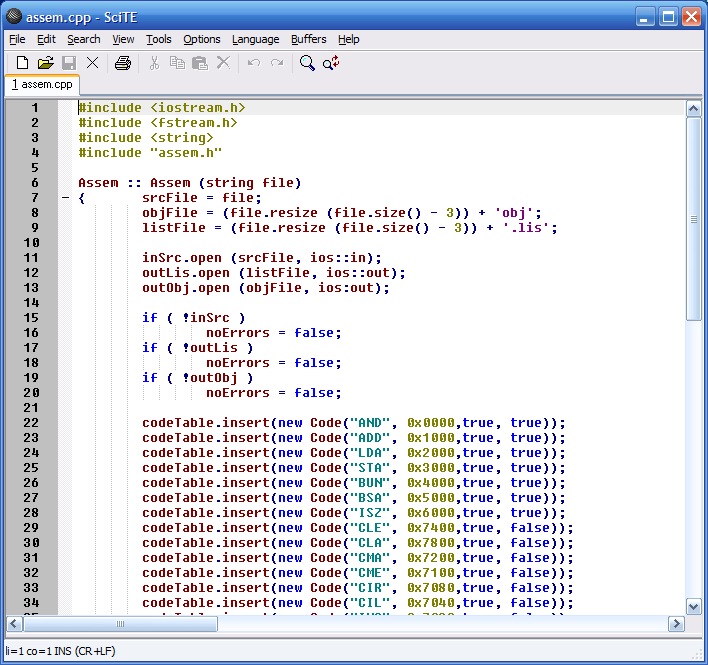
\includegraphics[width=0.7\textwidth]{images/scite.png}
\caption{Scintilla's syntax highlighting capabilities in the SciTE editor}
\label{fig:fig2,1.}
\end{figure}